\documentclass[../manual.tex]{subfiles}


\begin{document}
The GUI at its core is a chromium web instant that load a single JavaScript page application. The GUI is only necessary to communicate user input and retrieve result from back-end. It is not needed if the user only want to run the back-end.\par

\section{Back-end Connection}
At the top right is a button that can be used to access the back-end connection management windows where the user can start an instant of the Python back-end and manually adding more server connections to split user's the workload.\par

\begin{figure}[h]
	\centering
	\begin{framed}
		\centering
		
\includegraphics{connector-button}
		\caption{Button for access to the back-end connector management panel.}\label{fig:connectorbutton}
	\end{framed}
\end{figure}

The connector management panel has two sections. The first section is for running an instance of the back-end on the current computer. The input requires the absolute file path to the python binary that have access to Tornado v5+ and Pyteomics v3.5.1+, and the port number that the program would be run on.\par

In the second section of the panel, the user can enter addresses to one or more SWATHlib back-end instance. The GUI would check every saved addresses for accessibility by performing a GET request to the address at the path \emph{/api/swathlib/upload/} . If the response status is 200, the address is accessible else, it would be inaccessible and would not be used in the workflow.\par 

\section{User Input}
The GUI accepts protein sequences in FASTA format either in raw text or a text file. The user can perform in-silico trypsin digestion of the input with optional ability to manually or automatically select sites for misdigestion.\par

\subsection{Modification Customization}
Within user settings tab, the user can use their own table of modifications in tabular text file format as modifications source for the program. The table is made up of 10 columns where,\par

\begin{itemize}
	\item \textbf{name} is the name of the modification to be displayed on the GUI.
	\item \textbf{label} is the internal label of the modification to be used by the back-end. Must be in lowercase. No modifications within the same query should have the same label beside transition of the same Ytype variable modification.
	\item \textbf{mass} is the mass of the modification.
	\item \textbf{regex} is the regular expression representation of the the modification.
	\item \textbf{type} is the modification type \emph{Ytype}, \emph{variable}, or \emph{static}.
	\item \textbf{Ytype} is the label of the Ytype transition. Only applicable if type is Ytype.
	\item \textbf{multiplepattern} is whether the query with this variable modification is default to have all modification pattern generated. Only applicable if type is Ytype or variable.
	\item \textbf{status} is whether the query with this variable modification is default to be filled in every instance on the sequence. Only applicable if type is Ytype or variable.
	\item \textbf{mlabel} is the label for static modification in the annotated sequence.
	\item \textbf{offset} is the value offset for motif finding in case the digested fragments are cut within the motif. Only applicable with the GUI tryptic digestion tool.
\end{itemize}
\begin{table}[h]
	\caption{Example of a user submitted modifications table}
	\begin{adjustbox}{width=1\textwidth}
		\small
		\begin{tabular}{c c c c c c c c c c}
			\hline name   & label & mass      & regex           & type     & Ytype & multiplepattern & status & mlabel & offset \\ [0.1ex]
			\hline\hline
			O-Mannose     & g     & 0         & [S$|$T]         & Ytype    & Y0    & false           & false  &        & 0      \\
			O-Mannose     & g     & 162.05    & [S$|$T]         & Ytype    & Y1    & false           & false  &        & 0      \\
			HexNAc        & h     & 0         & N[\^{}P][S$|$T] & Ytype    & Y0    & false           & false  &        & 2      \\
			Propionamide  & c     & 71.037114 & C               & static   &       & false           & false  & PPa    & 0      \\
			Carboxylation & e     & 43.98983  & E               & variable &       & false           & false  &        & 0      \\
		\end{tabular}
	\end{adjustbox}
\end{table}

\subsection{SWATH Window Customization}
Similar to modification customization, the same settings tab, the user can also replace the default SWATH windows with an array of customized range using a tabular text file with two column, the first is the starting m/z of the windows while the second column is the stopping m/z of the windows.
\begin{table}[h]
	\caption{Example of a user submitted SWATH window table}
	\centering
	\begin{tabular}{c c}
		\hline start & stop \\
		\hline\hline
		400          & 425  \\
		424          & 450  \\
		449          & 475  \\
		474          & 500  \\
		499          & 525  \\
		524          & 550  \\
		549          & 575  \\
		574          & 600  \\
		599          & 625  \\
		624          & 650  \\
		649          & 675  \\
		674          & 700  \\
		699          & 725  \\
	\end{tabular}
\end{table}

\subsection{Retention Time Customization}
Within the user settings tab, a customized retention time list could be entered into the text box, each RT separated by a newline. Upon saving, the customized time would replace the default time within the GUI. Currently we only support time in integer.

\subsection{Main Input Settings}
Main input settings composed of 10 input parameters.\par

\begin{itemize}
	\item \textbf{Static Modifications}, modifications that will always be on the precursor sequences.
	\item \textbf{Non Ytype Variable Modifications}, variable modification that is not Ytype and may or may not appear on its supposed modification sites on the precursor sequences.
	\item \textbf{Ytype Variable Modifications}, variable modification that is Ytype and may and may or may not appear on its supposed modification sites on the precursor sequences. Multiple Ytype transition of the same modification can be applied without raising modification conflict issues.
	\item \textbf{Retention Time}, retention time for the library to be generated at.
	\item \textbf{SWATH Windows}, SWATH windows for the library to be generated at.
	\item \textbf{Max Charge}, max transition charge for the library to be generated at.
	\item \textbf{Precursor Charge}, charge of the precursor, only used in calculation of precursor m/z if no SWATH windows were selected.
	\item \textbf{Oxonium Ions}, ion fragments of a Ytype modification.
	\item \textbf{Fragmentation ion-type}, can be a string combination of \emph{b}, \emph{y}, and \emph{Y}, dictate which transition series that the library would attempt to generate.
	\item \textbf{Output Sequence Format At Variable Modifications}, dictate how the precursor annotated sequences would be uniquely identified across different RT and SWATH windows combination from each other at positions of variable modifications or at the end of the sequence. The three option is RT or SWATH windows or RT and SWATH windows.
\end{itemize}

These settings would apply to all sequences selected by the user at the beginning upon clicking the \emph{Apply Modifications} button and replaced any settings set before.\par

\subsection{Individual Query Settings}
Beside the main settings, the user can also customize a few parameters for each individual query sequence.\par

\begin{figure}[h]
	\centering
	
	\begin{framed}
		\centering
		\begin{adjustbox}{width=1\textwidth}
			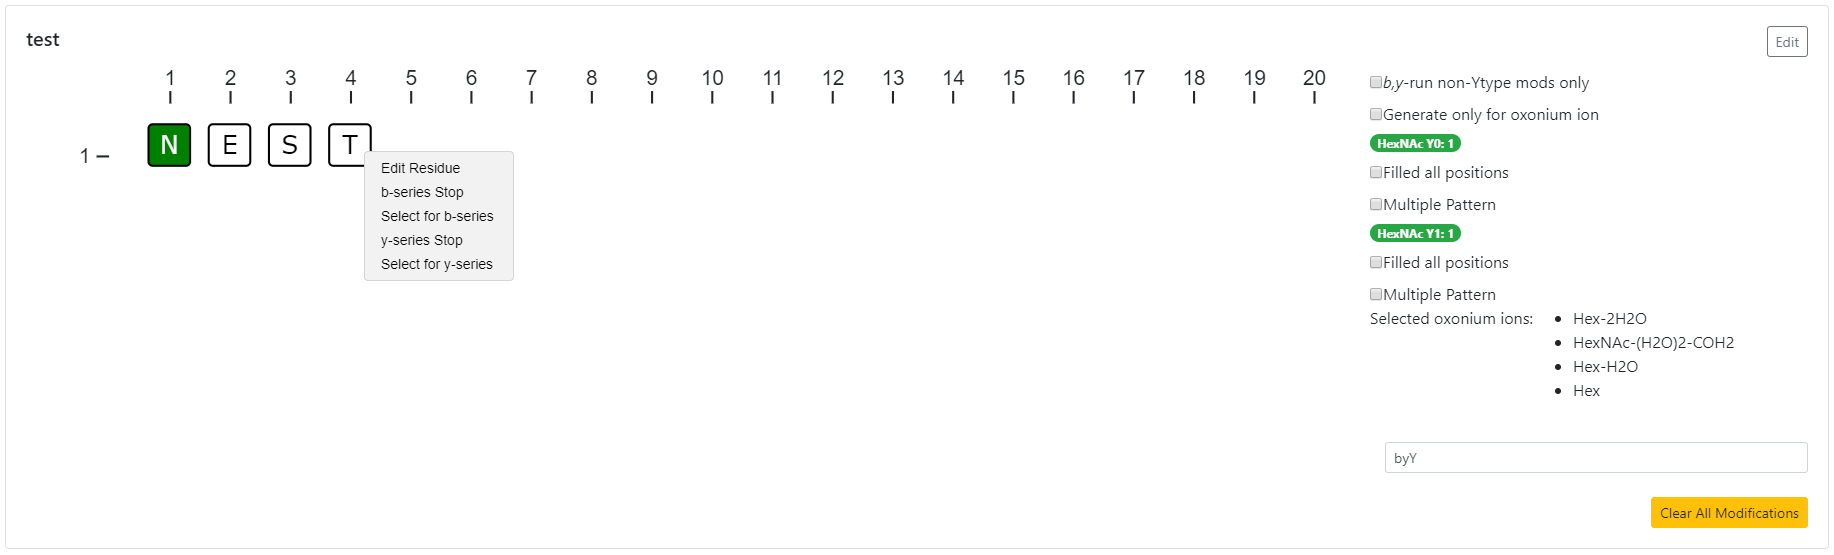
\includegraphics{individual-query}
		\end{adjustbox}
		\caption{Example of individual query.}\label{fig:individualquery}
	\end{framed}
	
\end{figure}

Each individual query panel is a graphical representation of the supplied sequence with modification from main settings applied to them. A context menu can be activate upon right clicking on each amino acid within the sequence with the following options\par
\begin{itemize}
	\item \textbf{Edit Residue}, allow direct customization with adding and removal of any modifications to the selected residue.
	\item \textbf{b-series Stop}, set this residue and all after it to not being generated for \emph{b} transition
	\item \textbf{Selected for b-series}, select this residue for b-series generation.
	\item \textbf{y-series Stop}, set this residue and all before it to not being generated for \emph{y} transition
	\item \textbf{Selected for y-series}, select this residue for y-series generation.
\end{itemize}

For variable modifications, the users can also select whether or not that they want the modifications to be either fill all sites or none (for non Ytype variable modifications) by checking the \textbf{Filled all positions} box. The box after that was for all possible modifications settings. If enable, it would generate all possible combination of this modifications across different identified modification sites. Depending on the complexity of the modifications and the length of the protein, if the \emph{b} and \emph{y} library can become quite large and it would also take a large amount of time to create.\par

The checkbox \textbf{b,y-run non-Ytype mods only} would disable Ytype modification mass from calculation of ion m/z for \emph{b} and \emph{y} transitions for this query.\par

If \textbf{Generate only for oxonium ion} is checked, only oxonium ions would be included for each unique precursor at each unique RT and SWATH window combinations.\par
\end{document}